‫
‫‫\section*{بخش تشریحی}
‫
‫الف) شمای ستاره‌ای در زمینهٔ ذخیره و سازماندهی داده‌ها به منظور تجزیه و تحلیل و گزارش‌دهی استفاده می‌شود. مزیت اصلی استفاده از شمای ستاره‌ای آسانی  تجزیه و تحلیل داده‌هاست. در شمای ستاره‌ای، داده‌ها به دو دسته‌ی اصلی تقسیم می‌شوند: \newline
‫۱) \LR{Fact table}: این جدول حاوی اطلاعات اصلی است. \newline
‫۲) \LR{Dimension tables}: این جداول حاوی اطلاعات توصیفی در مورد ابعاد مختلف داده‌های موجود در \LR{Fact table} هستند. \newline
‫با توجه به ساختار اصلی شمای‌ ستاره‌ای، برای ذخیره‌ی اطلاعات پروازهای خارجی این شما به شکل زیر می‌باشد.
‫
‫\begin{center}
‫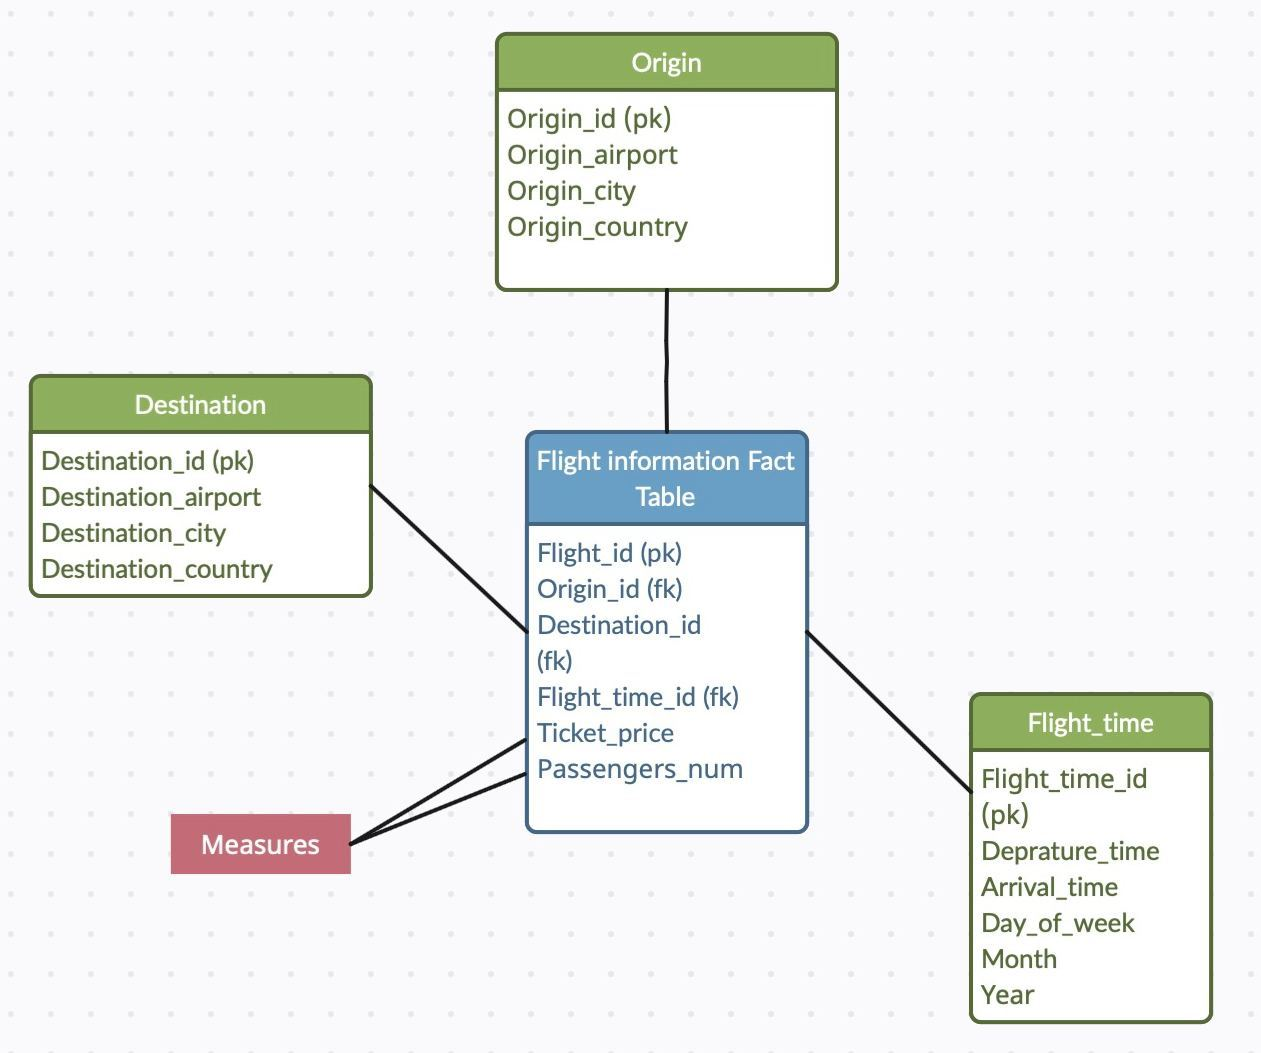
\includegraphics[scale=0.35]{figs/star_schema1.png}
‫\end{center}
‫
‫ویژگی‌های (attributes) هر کدام از بعدها در \LR{Dimension tables} خود آورده شده است. همچنین لازم به ذکر است که \LR{Flight_id} در \LR{Fact table} به عنوان کلید اصلی در نظر گرفته شده است. بسته به نیازی که تصور می‌شود می توان آن را حذف کرد یا نگه داشت. اما به صورت کلی وجود یک متغیر منحصر به فرد برای ثبت و پرس و جوی داده‌ها مناسب است.
‫\vspace{1cm}
‫
‫ب)  برای این مقایسه هر کدام از میانگین‌ها محاسبه و در پایان با یکدیگر مقایسه شده است. \newline
‫میانگین قیمت بلیط‌های تهران به میلان در خرداد ماه سال ۱۴۰۲: \newline
‫
\LR{\LR{Roll up on origin (from Origin-airport to Origin-city)} \newline
\LR{Roll up on Destination (from Destination-airport to Destination-city)} \newline
\LR{Roll up on Flight-time (from Departure-time to Month)} \newline
\LR{Dice for (Origin = “Tehran”) and (Destination = “Milan”)} \newline
\LR{Dice for (Flight-time = “Khordad”)} \newline
\LR{Roll up on Flight-time (from Month to Year)} \newline
\LR{Dice for (Flight-time = 1402)} \newline
\LR{Select AVG(Ticket-price)} \newline}

‫‫میانگین قیمت بلیط‌های تهران به آمستردام در فروردین ماه سال ۱۴۰۱: \newline
‫
\LR{\LR{Roll up on origin (from Origin-airport to Origin-city)} \newline
\LR{Roll up on Destination (from Destination-airport to Destination-city)} \newline
\LR{Roll up on Flight-time (from Departure-time to Month)} \newline
\LR{Dice for (Origin = “Tehran”) and (Destination = “Amesterdam”)} \newline
\LR{Dice for (Flight-time = “Farvardin”)} \newline
\LR{Roll up on Flight-time (from Month to Year)} \newline
\LR{Dice for (Flight-time = 1401)} \newline
\LR{Select AVG(Ticket-price)} \newline}
‫
‫\vspace{1cm}
‫
‫\hrule height .4 pt depth 0 pt width 16 cm \relax
‫
‫%------------------------------------------------------------------
‫
‫‫\section{سوال اول}
‫
‫
‫\vspace{1cm}
‫
‫\hrule height .4 pt depth 0 pt width 16 cm \relax
‫
‫%------------------------------------------------------------------
‫
‫\section{سوال دوم}
‫
‫
‫\vspace{1cm}
‫
‫\hrule height .4 pt depth 0 pt width 16 cm \relax
‫
‫‫%------------------------------------------------------------------
‫
‫\section{سوال سوم}
‫

‫\vspace{1cm}
‫
‫\hrule height .4 pt depth 0 pt width 16 cm \relax
‫
‫‫%------------------------------------------------------------------

‫\section{سوال چهارم}

‫\vspace{1cm}
‫
‫\hrule height .4 pt depth 0 pt width 16 cm \relax
‫
‫‫%------------------------------------------------------------------
‫
‫‫‫\section*{بخش عملی}
‫
‫